\section{Shamir's Secret Sharing}

Until now, we've only seen $n$-out-of-$n$ secret sharing schemes. The ``$n$-out-of-$n$'' part means that 
the reconstruction algorithm needs at least $n$ out of the $n$ total shares to recover the
secret; that is, it needs all of the shares to recover the secret. If the 
\share~algorithm outputs 2 shares, we need both shares to reconstruct.

In general, though, $(t+1)$-out-of-$n$ secret sharing schemes exist for any positive integers
$t$ and $n$.
($t$ stands for ``threshold'', since it determines the minimum number of parties necessary 
for reconstruction.)
In this section, we'll see how to construct such a secret sharing scheme using the properties 
of polynomials.

\subsection{Polynomials}

A \emph{polynomial} is an expression consisting of powers of a variable (or several variables,
but we'll stick with polynomials in one variable in this packet). Each power 
is multiplied by a number called its coefficient. Here's an example:
\[
    x^2 - 4x + 3
\]

The standard form for a polynomial in one variable (called a univariate polynomial) is 
\begin{equation}\label{eqn:std-form}
    a_n x^n + a_{n-1} x^{n-1} + \ldots + a_2 x^2 + a_1 x + a_0
\end{equation}

where the $a_n, \ldots, a_1$ are the coefficients of the polynomials. They 
are constant (fixed) values, usually integers. $n$ 
is a positive integer called the \emph{degree} of the polynomial. The example polynomial
above is a degree-2 polynomial.

% example polynomial graph
\begin{center}
\begin{tikzpicture}
\begin{axis}[
    axis x line=center,
    xlabel={$x$},
    axis y line=center,
    ylabel={$y$},
    xmin=-2.5,
    xmax=4.5,
    ymin=-2.5,
    ymax=7.5,
    grid,
    % ytick={-1,...,8},
]
\addplot[domain=-2:5,samples=50,mark=none,thick]{x^2-4*x+3};
% \node [right] at (axis cs: 4.5,0) {$x$};
% \node [above] at (axis cs: -1,11) {$f(x)$};
\node at (axis cs: 0,3) {\textbullet};
\node (coord) [above right,font=\small] at (axis cs: 0,3) {$(0,3)$};
\node [above right=-2mm and -10mm of coord,font=\small]  {$y$-intercept};
% \node (zero0) at (axis cs: 1,0) {\textbullet};
% \node (zero1) at (axis cs: 3,0) {\textbullet};
% \node (label) at (axis cs: 1,2) {zeroes};
% \draw[very thick,->] (label.south) to (zero0.north east);
% \draw[very thick,->] (label.south) to (zero1.north west);
\end{axis}
\end{tikzpicture}
% \caption{The graph of the polynomial $f(x)=x^1-4x+3$ with the $y$-intercept labeled.}
\end{center}

You may have plotted a polynomial before to show how its value changes 
with different values of $x$. A plot of our example polynomial is shown above.
In that case, we are plotting the equation 
\[
    f(x) = x^2 - 4x + 3
\]

where $f(x)$ is read as ``$f$ of $x$'' and indicates that the expression 
to the right of the equal sign is a function of the variable $x$. 

The \emph{$y$-intercept} of a function is the place where it crosses the $y$-axis, 
i.e. its value when $x=0$. In our example, the $y$-intercept is 3. Notice 
that we could have calculated it without plotting the equation:
\[
    f(0) = (0)^2 - 4(0) + 3 = 3
\]



When a polynomial is written in standard form as in Equation~\ref{eqn:std-form}, 
the $y$-intercept is $a_0$.

% The \emph{zeroes} of a function are the places where it crosses the $x$-axis,
% i.e. the values of $x$ for which $f(x)=0$. The zeroes in our example are 1 
% and 3:

% \begin{align*}
%     f(1) &= (1)^2 - 4(1) + 3 = 1 - 4 + 3 = 0\\
%     f(3) &= (3)^2 - 4(3) + 3 = 9 - 12 + 3 = 0
% \end{align*}

\begin{exercise}
    Write down the degree and $y$-intercept of each of the following 
    polynomials (without plotting them!):
    \renewcommand{\labelenumi}{(\alph{enumi})} 
    \begin{enumerate}
        \item $f(x) = x^2 + 3x - 1$
        \item $f(x) = 5x^2 + 11$
        \item $f(x) = -2x^3 - x^2 + 9x$
        \item $f(x) = 3x^5 - 2x^3 - 15$
        \item $f(x) = (x^2-1)(x+3)$
        \item $f(x) = 2(x-6)(x+2)(x-5)$
        \item $f(x) = 2x^3(x+16)$
    \end{enumerate}
\end{exercise}

\subsubsection{Uniqueness}\label{sec:unique}

An important property of polynomials is that we can describe any one 
polynomial with a set of points. If they meet a few simple conditions, 
these points will correspond to exactly one equation, so we say they 
\emph{uniquely define} that polynomial.

You've probably learned that two points uniquely define a line:

\begin{center}
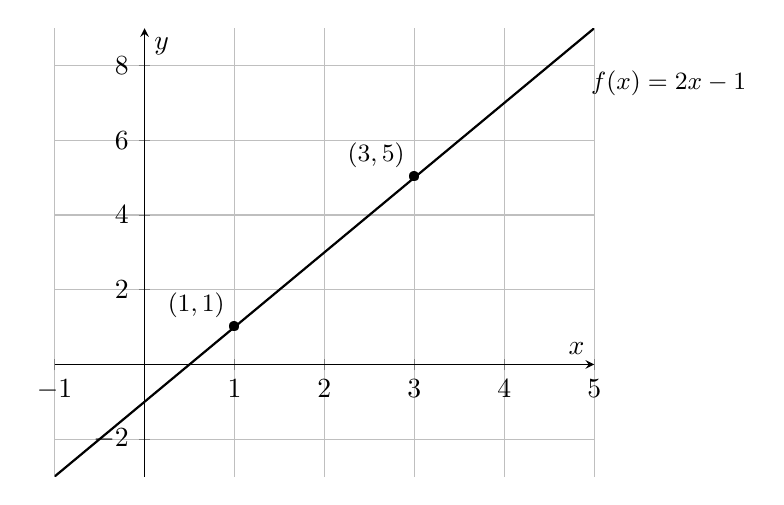
\begin{tikzpicture}
\begin{axis}[
    axis x line=center,
    xlabel={$x$},
    axis y line=center,
    ylabel={$y$},
    % xmin=-1.5,
    % xmax=5.5,
    % ymin=-1.5,
    % ymax=8.5,
    grid,
    % ytick={0,...,8},
]
\addplot[domain=-1:5,samples=50,mark=none,thick]{2*x-1};
\node (point1) at (axis cs: 1,1) {\textbullet};
\node [above left,font=\small] at (point1) {$(1,1)$};
\node (point2) at (axis cs: 3,5) {\textbullet};
\node [above left,font=\small] at (point2) {$(3,5)$};
\end{axis}
\node [font=\small] at (7.8,5) {$f(x)=2x-1$};
\end{tikzpicture}
\end{center}

In fact, we can view a line as a degree-1 polynomial, so we can uniquely 
define it via a set of points!
Instead of giving someone the equation for this line, you could 
give them 2 points on the line (for example, $(1,1)$ and $(3,5)$) and they'd 
still know exactly what line you're talking about. 

To specify a particular degree-2 polynomial, two points aren't enough.
For example, $x^2-4x+3$ goes through the points $(0,3)$ and $(4,3)$,
but so do many other degree-2 polynomials: 
%(represented here with dotted lines):

\begin{center}
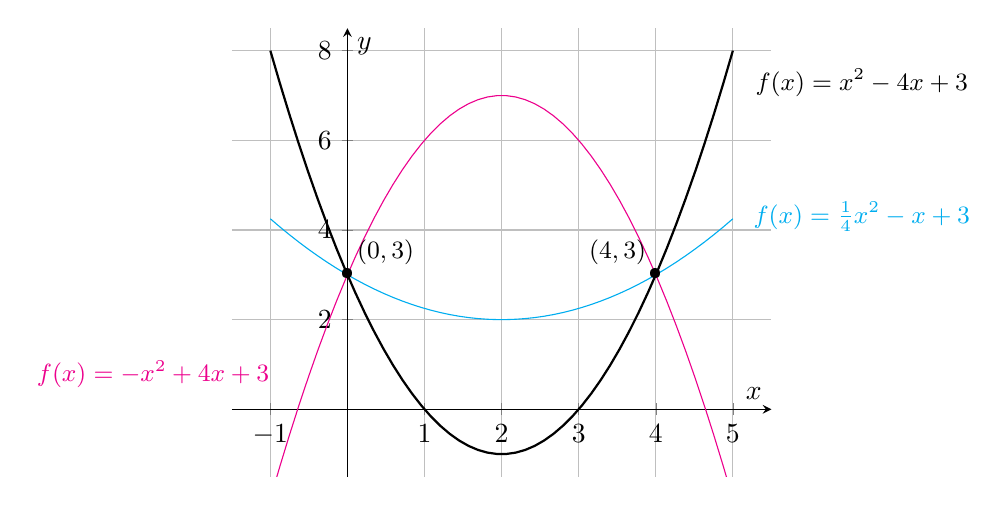
\begin{tikzpicture}
\begin{axis}[
    axis x line=center,
    xlabel={$x$},
    axis y line=center,
    ylabel={$y$},
    xmin=-1.5,
    xmax=5.5,
    ymin=-1.5,
    ymax=8.5,
    grid,
    % ytick={0,...,8},
]
\addplot[domain=-1:5,samples=50,mark=none,thick]{x^2-4*x+3};
% other degree-2 polys through these points
%%% BW VERSION %%%%%%
% \addplot[domain=-1:5,samples=50,mark=none,dotted]{-(x^2-4*x+3)+6};
% \addplot[domain=-1:5,samples=50,mark=none,dotted]{x^2/4-x+3};
%%% COLOR VERSION %%%%%
\addplot[domain=-1:5,samples=50,mark=none,magenta]{-(x^2-4*x+3)+6};
\addplot[domain=-1:5,samples=50,mark=none,cyan]{x^2/4-x+3};
% points (on top)
\node (point1) at (axis cs: 0,3) {\textbullet};
\node [above right,font=\small] at (point1) {$(0,3)$};
\node (point2) at (axis cs: 4,3) {\textbullet};
\node [above left,font=\small] at (point2) {$(4,3)$};
\end{axis}
\node [font=\small] at (8,5) {$f(x)=x^2-4x+3$};
\node [font=\small,magenta] at (-1,1.3) {$f(x)=-x^2+4x+3$};
\node [font=\small,cyan] at (8,3.3) {$f(x)=\frac{1}{4}x^2-x+3$};
\end{tikzpicture}
\end{center}

Instead, 3 points are needed to uniquely define a degree-2 polynomial:

\begin{center}
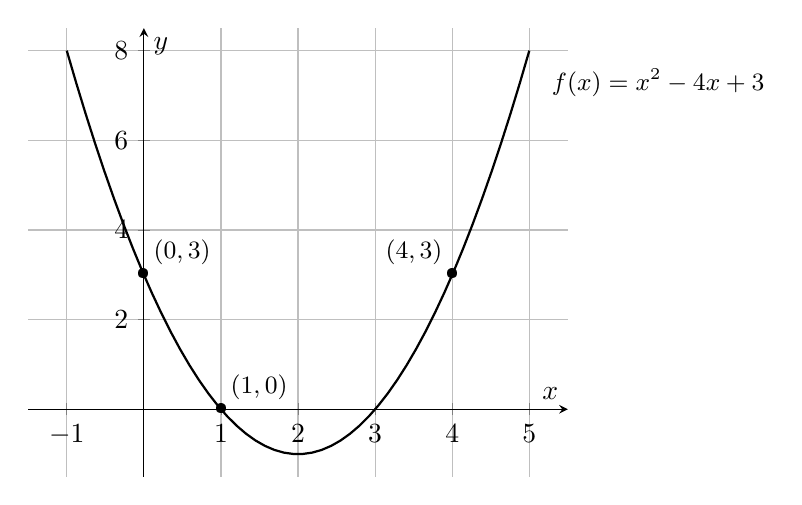
\begin{tikzpicture}
\begin{axis}[
    axis x line=center,
    xlabel={$x$},
    axis y line=center,
    ylabel={$y$},
    xmin=-1.5,
    xmax=5.5,
    ymin=-1.5,
    ymax=8.5,
    grid,
    % ytick={0,...,8},
]
\addplot[domain=-1:5,samples=50,mark=none,thick]{x^2-4*x+3};
\node (point1) at (axis cs: 0,3) {\textbullet};
\node [above right,font=\small] at (point1) {$(0,3)$};
\node (point2) at (axis cs: 4,3) {\textbullet};
\node [above left,font=\small] at (point2) {$(4,3)$};
\node (point3) at (axis cs: 1,0) {\textbullet};
\node [above right,font=\small] at (point3) {$(1,0)$};
\end{axis}
\node [font=\small] at (8,5) {$f(x)=x^2-4x+3$};
\end{tikzpicture}
\end{center}

How many points do you think are needed to uniquely define a degree-$n$
polynomial? Once you think you have an answer, flip to the next page.

\newpage
The process of recovering a polynomial passing through a set of points is 
called \emph{interpolation}. Accordingly, this general rule about the 
uniqueness of a polynomial described by a set of points is called the 
interpolation theorem:

\setlength\fboxsep{1em}        
\begin{center}
\fbox{
    \begin{minipage}{.7\linewidth}
        % \textbf{Interpolation Theorem.} \\
        \textsc{Interpolation Theorem.} \\
        Given a set of $t+1$ points, there 
        exists a unique degree-$t$ polynomial passing through those points.
    \end{minipage}
}
\end{center}

\begin{exercise}
    How many points are needed to uniquely define each polynomial 
    in the previous exercise?
\end{exercise}

If getting from a set of points to an equation sounds difficult, don't worry because 
there are well-known techniques that always work. Most programming languages 
actually have these built-in, so you don't need to know the details; you just 
plug points in and out comes a polynomial! In case you want to know more, though,
the next section explains how one of these techniques works.

\subsubsection{Lagrange Interpolation*}\label{sec:lagrange}

In this section we'll learn about one method of doing polynomial interpolation 
called \emph{Lagrange interpolation}. It's described by a single equation:

\begin{equation}\label{eqn:lagrange}
    P(x) = \sum_{i=0}^{m-1} y_i \ell_i(x), \text{ where } 
    \ell_i(x) = \prod_{\substack{j=0\\j\neq i}}^{m-1} \frac{x-x_j}{x_i-x_j}
\end{equation}

Let's break it down bit by bit. First, in case you aren't familiar with 
the symbols, $\sum_{i=0}^{m-1}$ is called \emph{summation notation} 
or \emph{sigma notation}. It means to evaluate the expression after 
$\sum$ for each value of $i$ (starting at the number below the summation 
symbol and ending at the number above) and then add all those terms together. For 
example:

\[
    \sum_{i=1}^m i = 1 + 2 + \ldots + m
\]

$\prod$ (\emph{product notation} or \emph{pi notation}) is similar, but we multiply the expressions instead of adding 
them:
\[
    \prod_{i=1}^m i = 1 \cdot 2 \cdot \ldots \cdot m
\]

So, $\sum_{i=1}^{4} i = 1+2+3+4 = 10$ and $\prod_{i=1}^4 i = 1 \cdot 2 \cdot 3 
\cdot 4 = 24$.

\begin{bonus}
    Evaluate the following expressions. Keep a close eye on the starting 
    value of $i$!
    \renewcommand{\labelenumi}{(\alph{enumi})} 
    \begin{enumerate}
        \item $\sum_{i=1}^5 2i$
        \item $\sum_{i=1}^5 1$
        \item $\sum_{i=0}^4 x_i$ where $x_i$ means the $i$th 
        elements of the set $\{1, 5, -3, 0, 8\}$ and the numbering
        starts at 0 (that is, $x_0=1$).
        \item $\sum_{i=0}^2 x_i$ for the same set.
    \end{enumerate}
\end{bonus}

\begin{bonus}
    Repeat the previous exercise, substituting $\prod$ for $\sum$.
\end{bonus}

Now, back to Lagrange interpolation. We start with a set of points $(x_0, y_0), 
\ldots,\allowbreak (x_n, y_n)$. For each point $(x_i, y_i)$, we compute the 
expression $\ell_i(x)$. For instance, for $i=2$, it will be of the form

\newcommand{\cyan}[1]{\textcolor{cyan}{#1}}
\[
    \setlength{\fboxsep}{.3\fboxsep}
    \frac{x-\boxed{x_0}}{x_2-\boxed{x_0}}
    \frac{x-\boxed{x_1}}{x_2-\boxed{x_1}}
    \frac{x-\boxed{x_3}}{x_2-\boxed{x_3}}
    \cdots
    \frac{x-\boxed{x_n}}{x_2-\boxed{x_n}}
\]

Then we plug that expression $\ell_i(x)$, along with the $y$-value $y_i$ 
for that point, into the summation, and we'll end up with a polynomial. 
If we did everything right, that will be exactly the polynomial defined 
by those points.

Let's work through an example using the degree-1 polynomial we plotted in Section~\ref{sec:unique}:
we'll use the points $(1,1), (3,5)$ to recover the equation of the line. Remember that,
in this packet, we start numbering the elements of a set at 0, so $(x_0,y_0)
= (1,1)$ and $(x_1, y_1) = (3,5)$.

\begin{example}
Use Lagrange interpolation to get a degree-1 polynomial passing through the points 
$(1,1), (3,5)$.

Since we have $2$ points, $m=2$:
\begin{align*}
    P(x) &= \sum_{i=0}^{1} y_i \ell_i(x)\\
    &= y_0 \ell_0(x) + y_1 \ell_1(x)
\end{align*}

Next, let's substitute in the $y$-coordinates of our points:
\[
    = 1 \cdot \ell_0(x) + 5 \cdot \ell_1(x)
\]

Now let's evaluate the polynomials $\ell_i(x)$:

\begin{align*}
    \ell_0(x) &= \prod_{\substack{j=0\\j\neq 0}}^{1} \frac{x-x_j}{x_0-x_j}\\
    &= \frac{x-x_1}{x_0-x_1}\\
    &= \frac{x-3}{1-3}
    = \frac{x-3}{-2}\\
    \ell_1(x) &= \prod_{\substack{j=0\\j\neq 1}}^{1} \frac{x-x_j}{x_1-x_j}\\
    &= \frac{x-x_0}{x_1-x_0}\\
    &= \frac{x-1}{3-1}
    = \frac{x-1}{2}
    % \ell_i(x) &= \prod_{\substack{j=0\\j\neq i}}^{n-1} \frac{x-x_j}{x_i-x_j}
\end{align*}

Plugging that back into the sum, we get

\begin{align*}
    P(x) &= 1 \cdot \ell_0(x) + 5 \cdot \ell_1(x)\\
    &= 1 \left(\frac{x-3}{-2}\right) + 5 \left(\frac{x-1}{2}\right)\\
    &= \frac{-(x-3)}{2} + \frac{5(x-1)}{2}\\
    &= \frac{5x-5-(x-3)}{2}\\
    &= \frac{4x-2}{2}
    = 2x-1\\
\end{align*}

That's the same equation as the one we graphed!
\end{example}

\begin{example}
Let's do the degree-2 example from Section~\ref{sec:unique} next. Our set of 
points is $\{(0,3),(1,0),(4,3)\}$ and $m=3$.
\begin{align*}
    P(x) &= \sum_{i=0}^{2} y_i \ell_i(x)\\
    &= y_0 \ell_0(x) + y_1 \ell_1(x) + y_2 \ell_2(x)\\
    &= 3 \cdot \ell_0(x) + 0 \cdot \ell_1(x) + 3 \cdot \ell_2(x)
\end{align*}

The polynomials $\ell_i(x)$ are:
\begin{align*}
    \ell_0(x) &= \prod_{\substack{j=0\\j\neq 0}}^{2} \frac{x-x_j}{x_0-x_j}\\
    &= \frac{x-x_1}{x_0-x_1} \frac{x-x_2}{x_0-x_2}\\
    &= \frac{x-1}{0-1} \frac{x-4}{0-4}\\
    &= \frac{x-1}{-1} \frac{x-4}{-4}
    = \frac{(x-1)(x-4)}{4}\\
\end{align*}
\begin{align*}
    \ell_1(x) &= \prod_{\substack{j=0\\j\neq 1}}^{2} \frac{x-x_j}{x_1-x_j}\\
    &= \frac{x-x_0}{x_1-x_0} \frac{x-x_2}{x_1-x_2}\\
    &= \frac{x-0}{1-0} \frac{x-4}{1-4}\\
    &= \frac{x}{1} \frac{x-4}{-3}
    = \frac{x(x-4)}{-3}\\
\end{align*}
\begin{align*}
    \ell_2(x) &= \prod_{\substack{j=0\\j\neq 2}}^{2} \frac{x-x_j}{x_2-x_j}\\
    &= \frac{x-x_0}{x_2-x_0} \frac{x-x_1}{x_2-x_1}\\
    &= \frac{x-0}{4-0} \frac{x-1}{4-1}\\
    &= \frac{x}{4} \frac{x-1}{3}
    = \frac{x(x-1)}{12}\\
    % \ell_i(x) &= \prod_{\substack{j=0\\j\neq i}}^{n-1} \frac{x-x_j}{x_i-x_j}
\end{align*}

Now we can simplify $P(x)$ to get:

\begin{align*}
    P(x) &= 3 \cdot \ell_0(x) + 0 \cdot \ell_1(x) + 3 \cdot \ell_2(x)\\
    &= 3 \cdot \frac{(x-1)(x-4)}{4} + 0 \cdot \frac{x(x-4)}{-3} + 3 \cdot \frac{x(x-1)}{12}\\
    &= \frac{3(x-1)(x-4)}{4} + \frac{3x(x-1)}{12}\\
    &= \frac{9(x-1)(x-4) + 3x(x-1)}{12}\\
    &= \frac{9(x^2-5x+4) + (3x^2-3x)}{12}\\
    &= \frac{9x^2-45x+36 + 3x^2-3x}{12}\\
    &= \frac{12x^2-48x+36}{12}\\
    &= x^2-4x+3
\end{align*}

and again we've arrived at the same polynomial we graphed.
\end{example}

\begin{bonus}
    Use Lagrange interpolation to find the unique degree-2 
    polynomial through the points $\{(-1,-16),(1,-2),(2,14)\}$.
\end{bonus}

\subsection{Sharing Secrets Using Polynomials}

Shamir secret sharing is a $(t+1)$-out-of-$n$ secret sharing scheme, for some positive integers $t$ and $n$. This means that we split the secret $s$ into $n$ values and distribute them to $n$ people. Then, at least $t+1$ of those people must work together to recover $s$.

Let's update our definition of secret sharing from Section~\ref{sec:formal-defs}
to include $(t+1)$-out-of-$n$ secret sharing schemes where $t+1 \neq n$.

% This is the (t+1)-out-of-n definition
\begin{definition}[Secret sharing scheme (updated)]\label{def:ss-update}
    Let $\D$ be the input domain and $\D_s$ be the share domain.
    A secret sharing scheme is a pair of efficient algorithms $(\share, \rec)$
    and two associated natural numbers $t,n$ such that

    \begin{itemize}
        \item \share~takes as input a secret $s \in \D$ and outputs $n$ 
        shares in $\D_s$.
        \item \rec~takes as input $m$ shares $s_1, \ldots, s_m \in D_s$ 
        and output some value $y \in \D$ or a special symbol $\perp$ 
        indicating failure. (If $m < t+1$, it outputs $\perp$.)
    \end{itemize}
\end{definition}

Now we're ready to put everything we've learned together and define 
Shamir's secret sharing scheme\footnotemark.
\footnotetext{Adi Shamir introduced this scheme in a short 1979 
paper entitled ``How to share a secret''\cite{shamir1979share}.
The paper is only two pages long, so if you're feeling adventurous 
you could have a go at it! You can find it online at 
\url{http://web.mit.edu/6.857/OldStuff/Fall03/ref/Shamir-HowToShareASecret.pdf}.}

\begin{figure}[h!]
\begin{pchstack}[center]
\fbox{%
\procedure{$\share(s)$}{%
    a_1, \ldots, a_t \sample \{1, \ldots, 2^\lambda\} \\
    a_0 = s\\
    f(x) = a_t x^t + \ldots + a_1 x + a_0\\
    \pcreturn ((1,f(1)), \ldots, (n,f(n)))
}
\pchspace
\procedure[space=auto]{$\rec(s_1, \ldots, s_m)$}{%
    \pcif m < t+1 \pcthen\\
    \pcreturn \perp\\
    \pcelse\\
    f(x) = \textsf{interpolate}(s_1, \ldots, s_m)\\
    \pcreturn f(0)
}
}
\end{pchstack}
\caption{Shamir's secret sharing scheme}
\label{fig:shamirSS}
\end{figure}

To share a secret $s$ in $\D$, we choose a random 
degree-$t$ polynomial $f$ by sampling $t$ random coefficients and 
setting $f$'s $y$-intercept to the secret. Then we pick $n$ points 
on $f$ (the convention is to evaluate $f$ at 1, 2, and so on, up 
to $n$)\footnotemark. These $n$ points are the shares.
\footnotetext{To be exact, Shamir's secret sharing evaluates $f$ 
in a way that ensures the values $f(x_i)$ are elements of something 
called a \emph{finite field}. We won't go into details here about 
what that means, since such polynomials can't be graphed in two 
dimensions, but just know that this is important for the scheme 
to be truly private.}

To reconstruct, we need at least $t+1$ points. The reconstruction 
algorithm takes these points $s_i = (x_i, y_i)$ and tries to recover 
$f$ using interpolation. (If there are not enough points, interpolation 
would fail, so we don't even try and instead return the symbol $\perp$ to indicate an error.)
Once we recover a polynomial, we evaluate it at 0 to find its 
$y$-intercept and output that.

\begin{example}
    Here's how we would compute $\share(12)$ with $t=1$ and $n=3$.
    First, we pick one random integer $a_1$, say $5$. Then $f(x)
    = 5x + 12$. Our three shares are $(1,17),(2,22),(3,27)$. Below 
    is a visual representation.
\end{example}

\begin{center}
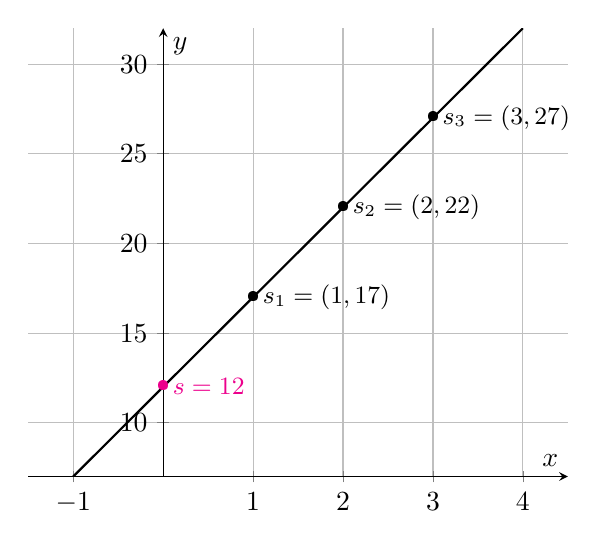
\begin{tikzpicture}
\begin{axis}[
    axis x line=center,
    xlabel={$x$},
    axis y line=center,
    ylabel={$y$},
    xmin=-1.5,
    xmax=4.5,
    % ymin=-2.5,
    % ymax=7.5,
    grid,
    % ytick={-1,...,8},
]
\addplot[domain=-1:4,samples=50,mark=none,thick]{5*x+12};
\node (share1) at (axis cs: 1,17) {\textbullet};
\node (share2) at (axis cs: 2,22) {\textbullet};
\node (share3) at (axis cs: 3,27) {\textbullet};
\node [right,font=\small] at (share1) {$s_1=(1,17)$};
\node [right,font=\small] at (share2) {$s_2=(2,22)$};
\node [right,font=\small] at (share3) {$s_3=(3,27)$};
\node [magenta] (s) at (axis cs: 0,12) {\textbullet};
\node [right,magenta,font=\small] at (s) {$s=12$};
\end{axis}
\end{tikzpicture}
\end{center}

\begin{example}
    Now let's say we receive two of the previous shares to reconstruct:
    $(1,17),(3,27)$. Say we know they are 2-out-of-3 shares (this is realistic; 
    in practice, $t$ and $n$ would be known to all the parties, or the 
    points would be labeled with the values of $t$ and $n$ used to 
    generate them.) How do we reconstruct?

    First of all, we know that reconstruction is possible because 
    we have $m=2$ shares and $t+1=2$, so $m \geq t+1$ as required for the 
    reconstruction algorithm not to fail immediately.
    Now we need to interpolate to recover the degree-2 polynomial 
    they represent. (If you didn't read Section~\ref{sec:lagrange}, 
    you can skip to the evaluation of $f(0)$ \todo{at the bottom of this page}.)

    Let's re-number the input shares starting with 
    0, so $(x_0,y_0) = (1,17)$ and $(x_1,y_1) = (3,27)$.
    \begin{align*}
        f(x) &= \sum_{i=0}^{m-1} y_i \ell_i(x)\\
        &= y_0 \ell_0(x) + y_1 \ell_1(x)\\
        &= 17 \ell_0(x) + 27 \ell_1(x)
    \end{align*}

    At this point, we can take a little shortcut. We know we only 
    care about finding the value of $f$ at 0, which means we only 
    need to find $\ell_0(0)$ and $\ell_1(0)$ instead of the full 
    expressions. So,
    \begin{align*}
        \ell_0(0) &= \prod_{\substack{j=0\\j\neq 0}}^{1} \frac{0-x_j}{x_0-x_j}
        = \frac{-3}{1-3}
        = \frac{3}{2}\\
        \ell_1(0) &= \prod_{\substack{j=0\\j\neq 1}}^{1} \frac{0-x_j}{x_1-x_j}
        = \frac{-1}{3-1}
        = -\frac{1}{2}
    \end{align*}

    % \begin{align*}
    %     f(x) &= 17 \ell_0(x) + 27 \ell_1(x)\\
    %     f(x) &= 17 \frac{x-2}{-1} + 27 \frac{x-1}{1}\\
    %     f(x) &= -17(x-2) + 27(x-1)\\
    %     f(x) &= -10x+7
    % \end{align*}
    Then 
    \begin{align*}
        f(0) &= 17 \ell_0(0) + 27 \ell_1(0)\\
        &= 17 \cdot \frac{3}{2} + 27 \cdot -\frac{1}{2}\\
        &= \frac{51-27}{2}\\
        &= \frac{24}{2} = 12\\
    \end{align*}
\end{example}

\begin{bonus}\label{bon:rec-groups}
    Work in a small group. Everyone in the group should pick 
    a secret number to share. Let $n$ be the number of people in 
    your group and pick $t$ so that $t+1 < n$. Use \share~to 
    compute shares of your secret and give each person in the group
    one share. Now a subgroup of $t+1$ people should work together 
    to reconstruct the secret using \rec\footnotemark. Once you succeed, 
    form a different group of $t+1$ people and run \rec~again
    using this new group of points. You should get the same 
    result!
    \footnotetext{You can use \url{https://www.dcode.fr/lagrange-interpolating-polynomial}
    to do the Lagrange interpolation.}
\end{bonus}

Notice that in the scheme presented in Figure~\ref{fig:shamirSS},
it's possible for someone to lie about their point, thereby 
causing the interpolation algorithm to return a different 
polynomial besides $f$. In that case, $f(0)$ might not equal $s$ 
and we'd recover the wrong secret!

This doesn't violate correctness, however, because in that case 
we aren't running \rec~on outputs of the \share~algorithm, so 
the correctness definition doesn't apply. Instead, what's happening 
is that our scheme fails when the parties don't behave honestly.
In cryptography, we say that the scheme is only secure in the 
presence of \emph{semi-honest} adversaries (the scheme has 
\emph{semihonest security}.) There are ways of fixing this scheme 
to guarantee security against \emph{malicious} adversaries 
(\emph{malicious security}), but that's outside the scope of this 
packet.

\begin{exercise}
    Visit \url{https://bit.ly/ShamirSS} in your browser. This is a 
    Google Colab notebook written in the Python programming language. 
    It already has the functions \share~and \rec~from Shamir's secret 
    sharing scheme. Work through the examples in the notebook to 
    share and reconstruct any numbers you want using this scheme, 
    then read on to find out how to share secret messages!
\end{exercise}

% TODO: if we use this exercise, must explain why $f$ needs to 
% be evaluated over a finite field
% \begin{bonus}
%     Show that Shamir secret sharing is private. (You can refer back to Section~\ref{sec:proof}
%     if necessary.)
% \end{bonus}
